% Options for packages loaded elsewhere
% Options for packages loaded elsewhere
\PassOptionsToPackage{unicode}{hyperref}
\PassOptionsToPackage{hyphens}{url}
%
\documentclass[
  a4paper,
]{article}
\usepackage{xcolor}
\usepackage[top=20mm,bottom=20mm,left=20mm,right=20mm]{geometry}
\usepackage{amsmath,amssymb}
\setcounter{secnumdepth}{-\maxdimen} % remove section numbering
\usepackage{iftex}
\ifPDFTeX
  \usepackage[T1]{fontenc}
  \usepackage[utf8]{inputenc}
  \usepackage{textcomp} % provide euro and other symbols
\else % if luatex or xetex
  \usepackage{unicode-math} % this also loads fontspec
  \defaultfontfeatures{Scale=MatchLowercase}
  \defaultfontfeatures[\rmfamily]{Ligatures=TeX,Scale=1}
\fi
\usepackage{lmodern}
\ifPDFTeX\else
  % xetex/luatex font selection
\fi
% Use upquote if available, for straight quotes in verbatim environments
\IfFileExists{upquote.sty}{\usepackage{upquote}}{}
\IfFileExists{microtype.sty}{% use microtype if available
  \usepackage[]{microtype}
  \UseMicrotypeSet[protrusion]{basicmath} % disable protrusion for tt fonts
}{}
\makeatletter
\@ifundefined{KOMAClassName}{% if non-KOMA class
  \IfFileExists{parskip.sty}{%
    \usepackage{parskip}
  }{% else
    \setlength{\parindent}{0pt}
    \setlength{\parskip}{6pt plus 2pt minus 1pt}}
}{% if KOMA class
  \KOMAoptions{parskip=half}}
\makeatother
% Make \paragraph and \subparagraph free-standing
\makeatletter
\ifx\paragraph\undefined\else
  \let\oldparagraph\paragraph
  \renewcommand{\paragraph}{
    \@ifstar
      \xxxParagraphStar
      \xxxParagraphNoStar
  }
  \newcommand{\xxxParagraphStar}[1]{\oldparagraph*{#1}\mbox{}}
  \newcommand{\xxxParagraphNoStar}[1]{\oldparagraph{#1}\mbox{}}
\fi
\ifx\subparagraph\undefined\else
  \let\oldsubparagraph\subparagraph
  \renewcommand{\subparagraph}{
    \@ifstar
      \xxxSubParagraphStar
      \xxxSubParagraphNoStar
  }
  \newcommand{\xxxSubParagraphStar}[1]{\oldsubparagraph*{#1}\mbox{}}
  \newcommand{\xxxSubParagraphNoStar}[1]{\oldsubparagraph{#1}\mbox{}}
\fi
\makeatother


\usepackage{longtable,booktabs,array}
\usepackage{calc} % for calculating minipage widths
% Correct order of tables after \paragraph or \subparagraph
\usepackage{etoolbox}
\makeatletter
\patchcmd\longtable{\par}{\if@noskipsec\mbox{}\fi\par}{}{}
\makeatother
% Allow footnotes in longtable head/foot
\IfFileExists{footnotehyper.sty}{\usepackage{footnotehyper}}{\usepackage{footnote}}
\makesavenoteenv{longtable}
\usepackage{graphicx}
\makeatletter
\newsavebox\pandoc@box
\newcommand*\pandocbounded[1]{% scales image to fit in text height/width
  \sbox\pandoc@box{#1}%
  \Gscale@div\@tempa{\textheight}{\dimexpr\ht\pandoc@box+\dp\pandoc@box\relax}%
  \Gscale@div\@tempb{\linewidth}{\wd\pandoc@box}%
  \ifdim\@tempb\p@<\@tempa\p@\let\@tempa\@tempb\fi% select the smaller of both
  \ifdim\@tempa\p@<\p@\scalebox{\@tempa}{\usebox\pandoc@box}%
  \else\usebox{\pandoc@box}%
  \fi%
}
% Set default figure placement to htbp
\def\fps@figure{htbp}
\makeatother





\setlength{\emergencystretch}{3em} % prevent overfull lines

\providecommand{\tightlist}{%
  \setlength{\itemsep}{0pt}\setlength{\parskip}{0pt}}



 


\makeatletter
\@ifpackageloaded{caption}{}{\usepackage{caption}}
\AtBeginDocument{%
\ifdefined\contentsname
  \renewcommand*\contentsname{Table of contents}
\else
  \newcommand\contentsname{Table of contents}
\fi
\ifdefined\listfigurename
  \renewcommand*\listfigurename{List of Figures}
\else
  \newcommand\listfigurename{List of Figures}
\fi
\ifdefined\listtablename
  \renewcommand*\listtablename{List of Tables}
\else
  \newcommand\listtablename{List of Tables}
\fi
\ifdefined\figurename
  \renewcommand*\figurename{Figure}
\else
  \newcommand\figurename{Figure}
\fi
\ifdefined\tablename
  \renewcommand*\tablename{Table}
\else
  \newcommand\tablename{Table}
\fi
}
\@ifpackageloaded{float}{}{\usepackage{float}}
\floatstyle{ruled}
\@ifundefined{c@chapter}{\newfloat{codelisting}{h}{lop}}{\newfloat{codelisting}{h}{lop}[chapter]}
\floatname{codelisting}{Listing}
\newcommand*\listoflistings{\listof{codelisting}{List of Listings}}
\makeatother
\makeatletter
\makeatother
\makeatletter
\@ifpackageloaded{caption}{}{\usepackage{caption}}
\@ifpackageloaded{subcaption}{}{\usepackage{subcaption}}
\makeatother
\usepackage{bookmark}
\IfFileExists{xurl.sty}{\usepackage{xurl}}{} % add URL line breaks if available
\urlstyle{same}
\hypersetup{
  pdftitle={3. Series AC Circuits},
  hidelinks,
  pdfcreator={LaTeX via pandoc}}


\title{3. Series AC Circuits}
\author{}
\date{}
\begin{document}
\maketitle

\renewcommand*\contentsname{Table of contents}
{
\setcounter{tocdepth}{3}
\tableofcontents
}

\subsection{Circuits}\label{circuits}

In a series circuit, in place of \(R\), we use \(Z\): -
\(Z_T = Z_1 + Z_2 + Z_3 \dots\)

\subsubsection{Resistors}\label{resistors}

For a circuit with a resistor and ac source: -
\(i = I \sin \omega t = I \angle 0^\circ, \text{ where } I = I_m\) -
\(Z = R \angle 0^\circ\)

\subsubsection{Inductors}\label{inductors}

For a circuit with an inductor and an AC source: -
\(i = I_m \sin (\omega t -90^\circ) = I\angle -90^\circ\), when
\(v = V \angle 0^\circ\) - \(v = V\angle 90^\circ\), when
\(i = I \angle 0^\circ\) - \(Z = X_L \angle 90^\circ\)

\subsubsection{Capacitors}\label{capacitors}

For a circuit with a capacitor and an AC source:

\begin{itemize}
\item
  \(i = I_m \sin (\omega t + 90^\circ) = I\angle 90^\circ\), when
  \(v = V \angle 0^\circ\)
\item
  \(v = V\angle -90^\circ\), when \(i = I \angle 0^\circ\)
\item ~
  \subsection{\texorpdfstring{\(Z = X_C \angle -90^\circ\)}{Z = X\_C \textbackslash angle -90\^{}\textbackslash circ}}\label{z-x_c-angle--90circ}

  \begin{center}\rule{0.5\linewidth}{0.5pt}\end{center}

  \subsection{RLC circuit}\label{rlc-circuit}
\end{itemize}

In an \(RLC\) circuit, depending on the value of the resistance and
reactances, the circuit is resistive, inductive or capacitive.

\subsubsection{Impedence Diagram}\label{impedence-diagram}

\begin{figure}[H]

{\centering \pandocbounded{\includegraphics[keepaspectratio]{images/image-1.png}}

}

\caption{image}

\end{figure}%

\begin{quote}
\textbf{ⓘ Note} \(Z_C \neq X_C\angle90^\circ\)
\(Z_C = X_C\angle-90^\circ\)
\end{quote}

For any configuration, the angle associated with the total impedance is
the angle by which the applied voltage leads the source current.

\begin{longtable}[]{@{}ll@{}}
\toprule\noalign{}
Network & \(\theta_{Z_T}\) \\
\midrule\noalign{}
\endhead
\bottomrule\noalign{}
\endlastfoot
Inductive & \(+ve\) \\
Capacitive & \(-ve\) \\
\end{longtable}

\subsubsection{Series ac Circuits
(Configurations)}\label{series-ac-circuits-configurations}

Impedances behave like resistors in series. \[Z_T = \sum Z_n\]

Calculating in complex mode (recommended to use):

\begin{quote}
\textbf{ⓘ Note} In all places, angles are required in equations except
in avg power formula (\(P=VI\cos\theta\)). Each attribute has its own
angle except avg power
\end{quote}

\begin{itemize}
\item
  Polar notation \[
  \begin{align*}
    E &= I \cdot Z_T \\
    I &= \frac{E}{Z_T} \\
    V_{Z_x} &= I_T \cdot Z_x \\
    I_{Z_x} &= I \\
  \end{align*}
  \]
\item
  Rectangular notation
\end{itemize}

\[
\begin{align*}
    Z &= R+j(X_L-X_C) \\
\end{align*}
\]

Calculating in non-complex mode (not recommended to use):

\[
\begin{align*}
    Z &= \sqrt{R^2+X} \\
    X &= X_L-X_C\\
    \theta &= \tan^{-1} \frac{X}{R} \\
\end{align*}
\]

Calculations that are complex independant:

\(P=EI\cos\theta\)

\paragraph{Voltage Divider Rule}\label{voltage-divider-rule}

\(V_x = \dfrac{E}{Z_T}Z_x\)

\begin{quote}
\textbf{ⓘ Note} Basically, this is Ohm's law. The only change is that
\(I\) has been expanded
\end{quote}

\(V_x = I \cdot Z_x = \dfrac{E}{Z_T}Z_x\)

\paragraph{Kirchoff's Voltage Law}\label{kirchoffs-voltage-law}

The sum of the input voltages and voltage drops in a closed loop is zero

\subsubsection{Resonance}\label{resonance}

Condition for resonance:

\[X_L = X_C\]

Frequency:

\[f = \frac{1}{2\pi\sqrt{LC}}\]

Derivation for \(f\)

\begin{quote}
\textbf{ⓘ Note} This is very simple, use when you forget the formula for
\(f\), all you need to remember is the condition for resonace.
\end{quote}

\[
\begin{align*}
    X_L &= X_C \\
    \omega L &= \frac{1}{\omega C} \\
    2\pi fL &= \frac{1}{2\pi fC} \\
    f^2 &= \frac{1}{(2\pi)^2LC} \\
    f& = \frac{1}{2\pi\sqrt{LC}} \\
\end{align*}
\]

\subsubsection{Applying the general approach to a series RLC
circuit}\label{applying-the-general-approach-to-a-series-rlc-circuit}

\begin{itemize}
\tightlist
\item
  Apply the phasor notation
\end{itemize}

\begin{figure}[H]

{\centering \pandocbounded{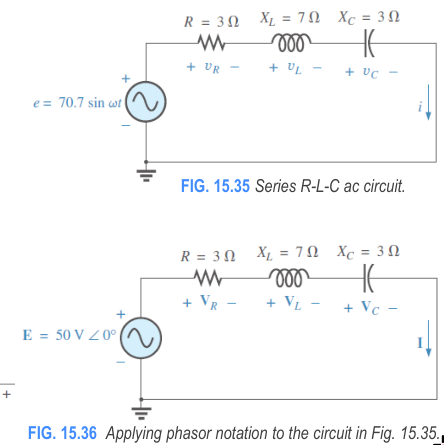
\includegraphics[keepaspectratio]{images/image-2.png}}

}

\caption{image}

\end{figure}%

\begin{itemize}
\item
  Calculate the total impedance of the circuit

  \begin{itemize}
  \tightlist
  \item
    \(Z_T = Z_R + Z_L + Z_C\)
  \end{itemize}
\item
  Draw: Impedance diagram
\item
  Determine the total current

  \begin{itemize}
  \tightlist
  \item
    \(I = \dfrac{E}{Z_T}\)
  \end{itemize}
\item
  Find the voltage across each element

  \begin{itemize}
  \tightlist
  \item
    \(V_R = IZ_R = (I\angle\theta)(R\angle 0^\circ)\)
  \item
    \(V_L = IZ_L = (I\angle\theta)(X_L\angle 90^\circ)\)
  \item
    \(V_C = IZ_C = (I\angle\theta)(X_C\angle -90^\circ)\)
  \end{itemize}
\item
  Apply Kirchoff's voltage law
  \(\sum V = E-V_R-V_L-V_C = 0 \text{ or } E = V_R+V_L+V_C\), verified
  through phasor diagram
\item
  Draw the phasor diagram
\item
  Determine the power to the circuit

  \begin{itemize}
  \tightlist
  \item
    \(P=V_mI_m\cos\theta\)
  \end{itemize}
\item
  Calculate the power factor

  \begin{itemize}
  \tightlist
  \item
    \(F_p = \cos \theta_T = \dfrac{R}{Z_T}\)
  \end{itemize}
\end{itemize}

\subsection{Frequency Response for Series ac
Circuits}\label{frequency-response-for-series-ac-circuits}

In a series R-L-C circuit: - At very low frequencies, the total
impedance will be determined primarily by the capacitor (C). - At very
high frequencies, the total impedance will be determined primarily by
the inductor (L).

\begin{figure}[H]

{\centering \pandocbounded{\includegraphics[keepaspectratio]{images/image-4.png}}

}

\caption{image}

\end{figure}%




\end{document}
